\documentclass[a4paper,10pt]{article}
\usepackage[T1]{fontenc}
\usepackage[utf8]{inputenc}
\usepackage{lmodern,textcomp}
\usepackage[margin=2.2cm]{geometry}
\usepackage{amsmath,amssymb,siunitx,booktabs,graphicx,tabularx,array,enumitem,xcolor,fancyhdr,float}
\usepackage[colorlinks=true,linkcolor=blue!50!black,urlcolor=blue!50!black]{hyperref}
\setlength{\parindent}{0pt}
\setlength{\parskip}{4pt}
\setlength{\headheight}{14pt}
\renewcommand{\arraystretch}{1.2}
\renewcommand{\tabularxcolumn}[1]{>{\raggedright\arraybackslash}p{#1}}
\setlist{nosep,leftmargin=*}
\newcommand{\file}[1]{\nolinkurl{#1}}
\sisetup{per-mode=symbol}
\pagestyle{fancy}\fancyhf{}
\fancyhead[L]{34870 Electroacoustics}
\fancyhead[R]{Lab C --- Microphone calibration}
\fancyfoot[L]{Group 10 \quad / \quad measured 29 September 2026}
\fancyfoot[R]{\thepage}
\graphicspath{{../figures/}{Lab C/figures/}{../ltspice/}{Lab C/ltspice/}}
\begin{document}
\begin{center}
{\Large\bfseries Lab E --- Loudspeaker response in free field}\\[5pt]
34870 Electroacoustics\\[4pt]
Group 10: Louis Andrianne, Sophie Kimura, Mads Rudolph\\[4pt]
Measured Tuesday 20 October 2026, building 354, room 026
\end{center}
\thispagestyle{fancy}

\section{Purpose and Setup}

The purpose of this lab is to illustrate how the frequency response and directivity of a loudspeaker unit depend on the shape of the baffle it is mounted on. This lab will measure responses across a small box, a circular screen, and an IEC screen to do this. Additionally, the purpose of this lab is to measure the frequency response of the units in the project loudspeaker system.\\

\textit{Setup here}

\section{Part 1: Effect of the Mounting Shape}

The ideal condition for measuring a loudspeaker driver is when it is mounted in an infinite baffle. This way, there is no diffraction around the edges of the baffle, as this can affect its radiation pattern. A semi-anechoic chamber with one fully reflective surface would be able to approximate an infinite baffle, as the reflective surface could act as the baffle. However, this lab takes place in a full anechoic chamber and so some approximation must be done. An asymmetric mounting on a finite size baffle helps minimize the diffraction coming from the edges, as the following lab will show.

\subsection{Measurement Procedure}

In this exercise, the internal sound card of the desktop PC in the control room is used. The output comes directly back in as input and also sent to the audio amplifier. The UMIK microphone is placed in the anechoic chamber and connected to the desktop as well. A Matlab measurement function is used to obtain the frequency vector and spectrum vector for both the input signal and the corresponding microphone signal, using the equation:

\begin{equation}
    H_{pv} = \frac{specn(:,2)}{specn(:,1)}
\end{equation}

for each element in $specn$. The frequency range goes from 50Hz to 20000Hz for all of the measurements in this section. The effective diameter of the 3-inch driver is derived from the rule of thumb that the piston radius in cm in around equal in number to the diameter in inches of the unit. This correlates to an effective diameter of 0.06 meters.

\subsection{Frequency response: Small box}

The transfer function for the loudspeaker in its small box is first measured, positioned at 0 degrees and 30 degrees from horizontal. 

\begin{figure}[H]
    \centering
    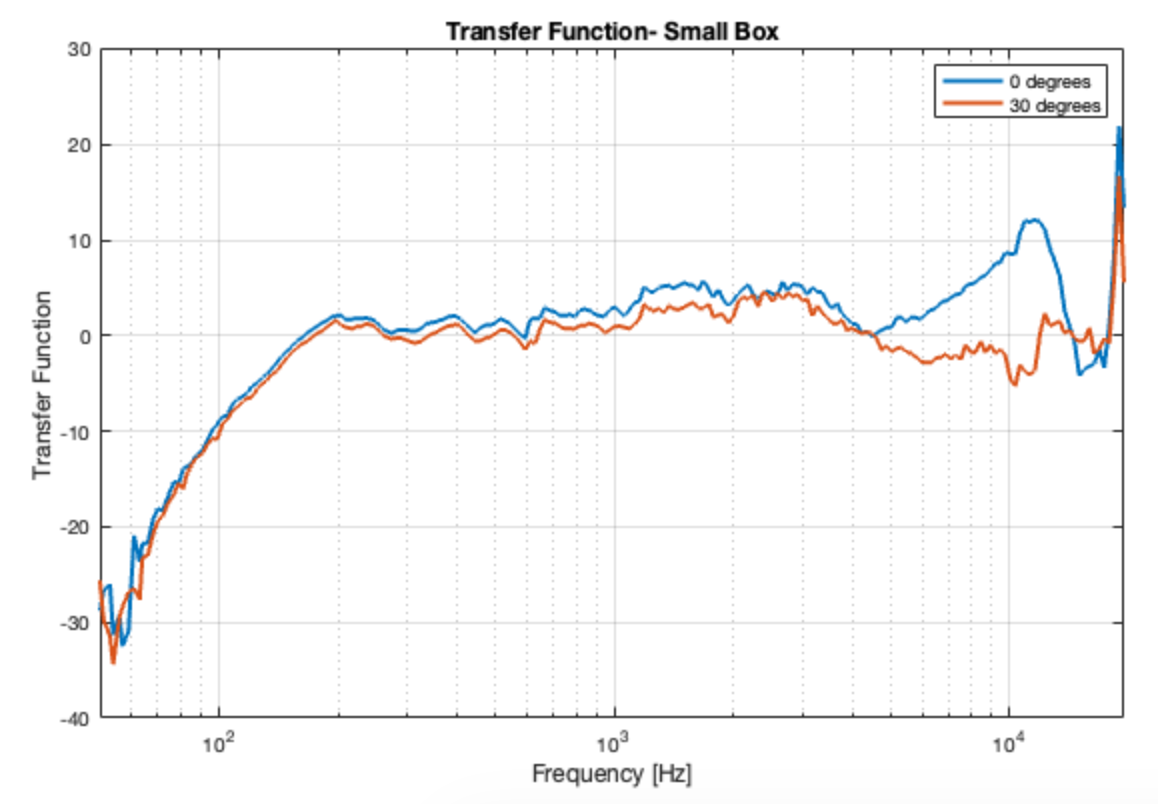
\includegraphics[width=0.6\linewidth]{Lab E/figures/smallbox.png}
    \caption{Small box}
    \label{fig:smallbox}
\end{figure}

The small box response is generally flat at low frequencies until around 400Hz at both 0 and 30 degrees. At this frequency, for the 0 degree configuration, there is a large spike in the response that reaches up to around 10dB, while it instead dips a little bit in the 30 degree configuration.

\subsection{Frequency response: Circular screen}

The circular screen is mounted onto the loudspeaker unit and is measured at 0 and 30 degrees. The screen radius is measured at 0.3 meters.

\begin{figure}[H]
    \centering
    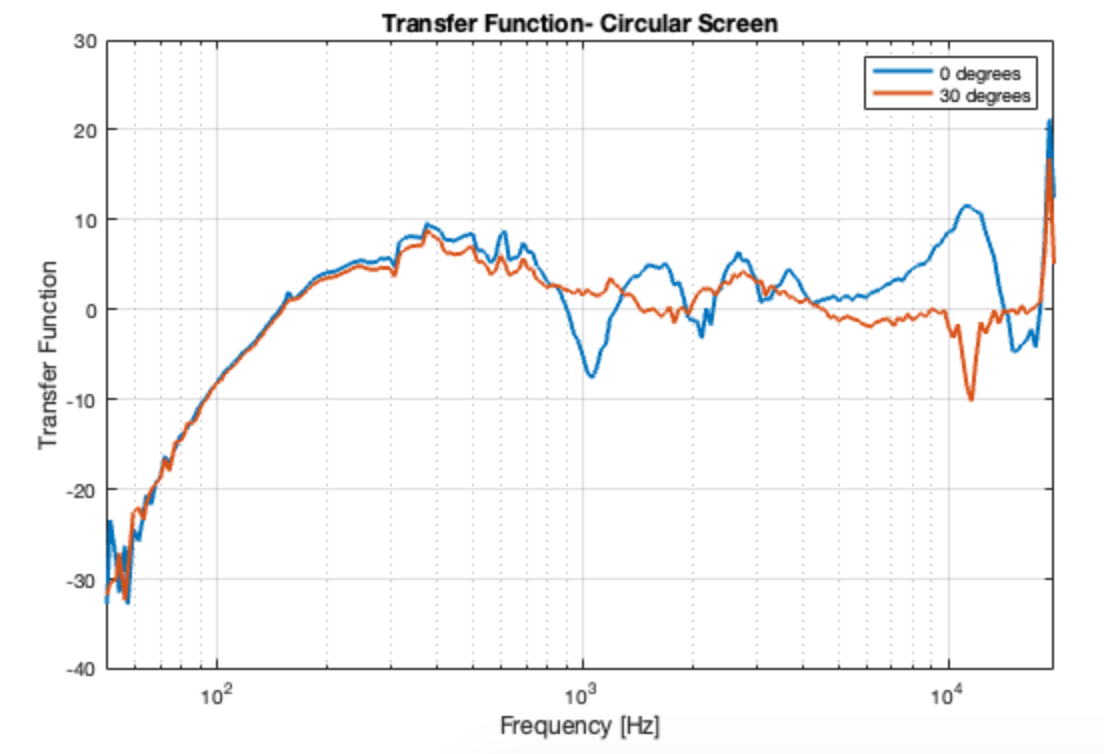
\includegraphics[width=0.6\linewidth]{Lab E/figures/circularscreen.png}
    \caption{Circular Screen}
    \label{fig:circularscreen}
\end{figure}

With the circular screen, the response does not revolve around the 0dB, but is a bit raised. The responses for the 0 and 30 degree configurations start to separate immediately in the low frequencies, with the 0 degree configuration having a higher dB. The 0 degree setup includes multiple resonances and antiresonances throughout the frequency spectrum, with four noticeable peaks. The 30 degree configuration instead shows less sharp peaks, but still includes buildups and drops, including a very sharp drop at around 1000Hz, when the 0 degree configuration has its sharpest peak.

\subsection{Frequency response: IEC screen}

The rectangular screen is mounted onto the setup with asymmetric speaker position and measured at 0, 15, 20, and 60 degrees.

\begin{figure}[H]
    \centering
    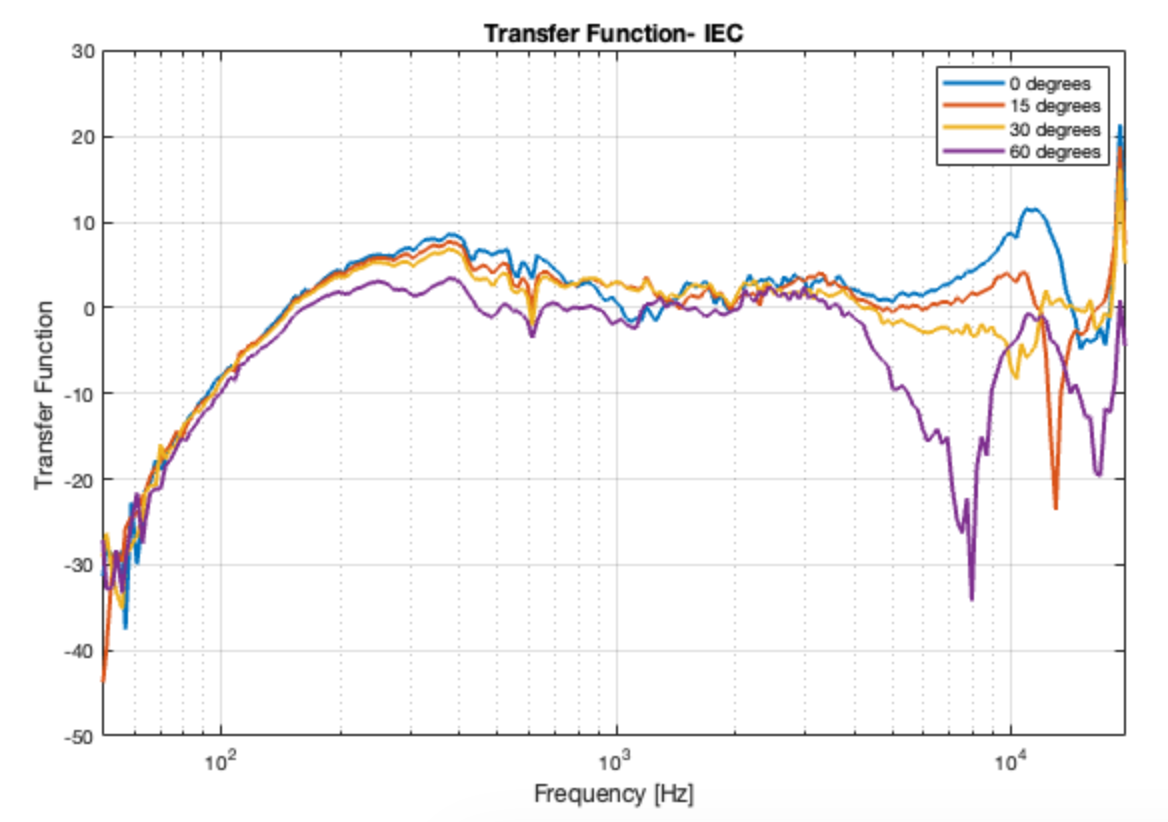
\includegraphics[width=0.6\linewidth]{Lab E/figures/iec.png}
    \caption{Rectangular screen}
    \label{fig:iec}
\end{figure}

\subsection{Analysis}

\begin{figure}[H]
    \centering
    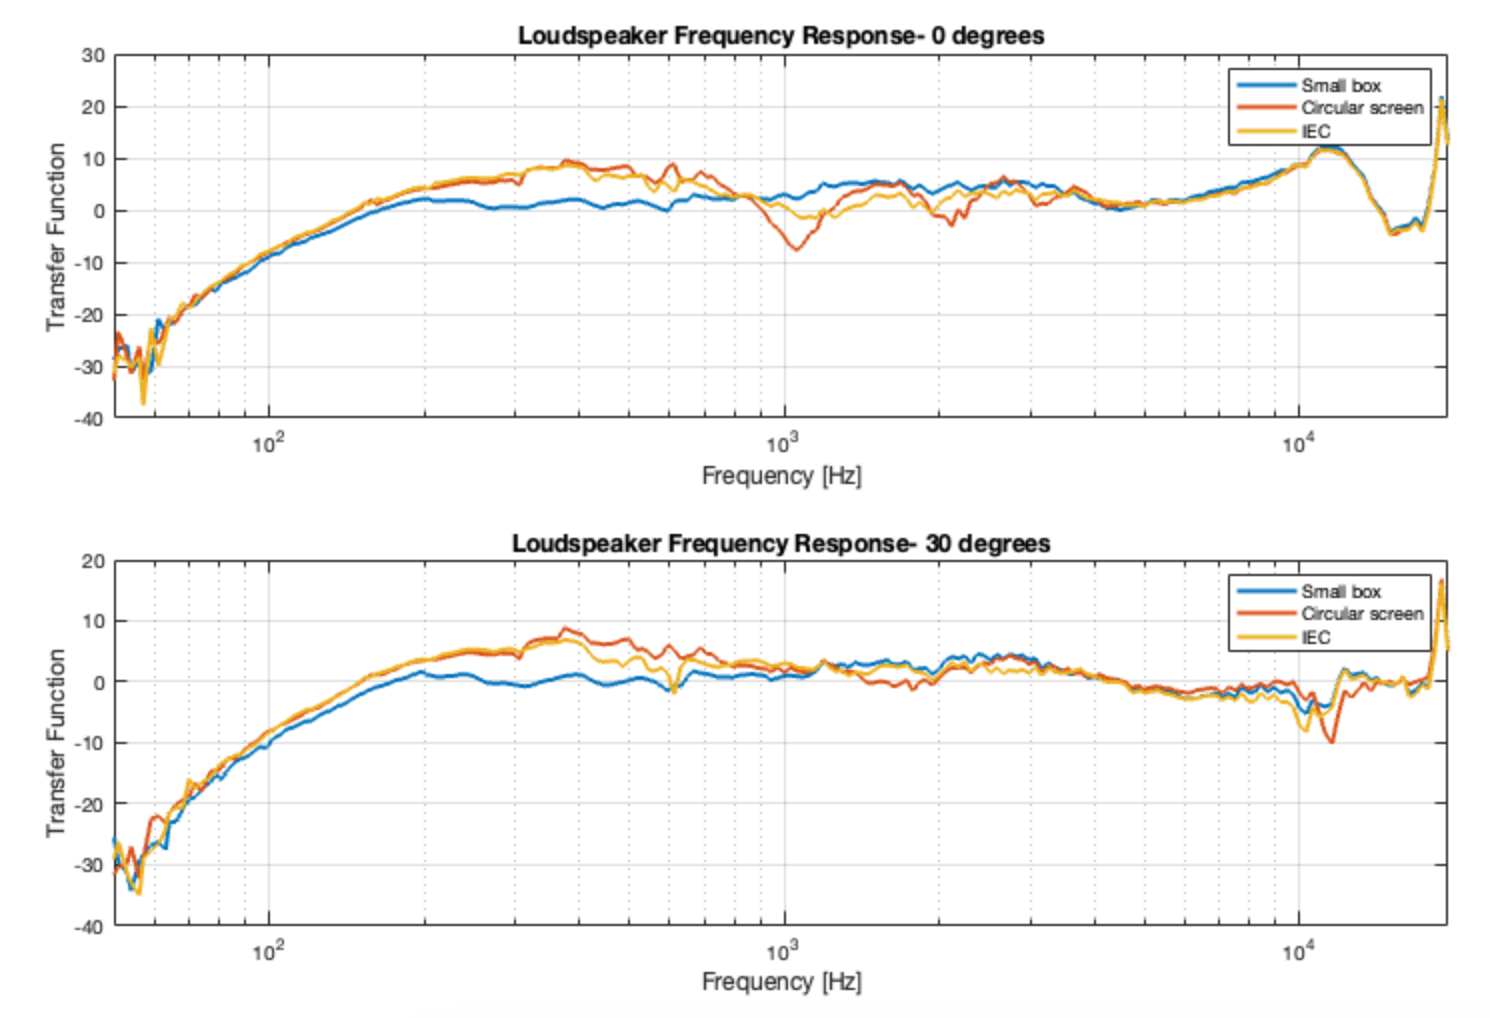
\includegraphics[width=0.8\linewidth]{Lab E/figures/3setups.png}
    \caption{Three setups compared}
    \label{fig:3setups}
\end{figure}

The frequency response for the small box is generally flat around 0dB for both throughout the region of interest, 125Hz to 20000Hz. In the lower frequencies up until around 1000Hz, the small box circular screen and IEC setups have a higher frequency response than the small box, across 0 and 30 degrees. They both dip a little below the small box response after this point. For the response at 0 degrees, the circular screen experiences dips which correspond with resonances and antiresonances. The IEC also goes below the small box response, but is a bit more flat. This is still true for the IEC at 30 degrees, while the circular screen changes behavior and has less sharp peaks. 

\section{Part 2: Project system anechoic measurement}

\subsection{Effective diameter of drivers}

\subsection{Frequency response: Drivers}

\subsection{Measurement procedure with sound card}

\subsection{Procedure for obtaining compensated plot of relative phases between drivers at 0 degrees}

\section{Conclusion}







\end{document}